\documentclass[portrait,fleqn,12pt]{beamer}
\usetheme[progressbar=frametitle]{metropolis}
\usepackage{amsmath}
\usepackage{fleqn,amssymb,shadow}
\usepackage{float}
\usepackage{epsfig}
\usepackage{enumerate}
\usepackage{cancel}
\usepackage{fontawesome5}
\usepackage{fourier}
\usepackage{upgreek}
%\raggedright

% Custom commands
\newcommand{\fma}{{\rm fma}}
\newcommand{\reals}{\mathbf{R}}
\newcommand{\epsmach}{\varepsilon_m}
\newcommand{\mymax}{\mbox{max} \,\,}
\newcommand{\mydeg}{\mbox{deg}}
\newcommand{\dom}{\mbox{dom}}
\newcommand{\fl}{\mbox{fl}}
\newcommand{\rel}{\mbox{rel}}
\newcommand{\cond}{\mbox{cond}}
\newcommand{\bern}{\mathcal{B}}
\newcommand{\order}{\mathcal{O}}
\newcommand{\atan}{\rm{arctan}}
\newcommand{\bfa}{\mathbf{a}}
\newcommand{\bfb}{\mathbf{b}}
\newcommand{\bfzero}{\mathbf{0}}
\newcommand{\bfx}{\mathbf{x}}
\newcommand{\complex}{\mathbf{C}}
\newcommand{\integers}{\mathbf{Z}}
\newcommand{\D}{\mathrm{D}}

% Custom environments
\newenvironment{alphalist}
   {\begin{enumerate}[(a)]
       \addtolength{\itemsep}{0.0\itemsep}}
     {\end{enumerate}}

\newenvironment{handlist}
   {\begin{enumerate}[\faHandPointRight]
       \addtolength{\itemsep}{0.0\itemsep}}
     {\end{enumerate}}

\newenvironment{define}[1]{
  \textbf{Definition} #1}{}

\newenvironment{idefine}[2]{
  \index{#1}
  \textbf{Definition} #2}{\(\blacktriangleleft\)}

\newenvironment{myexample}[1]{
  \textbf{Example} #1}


\newenvironment{mynote}[1]{
  \textbf{Note} #1}

\begin{document}

\begin{frame}
\begin{flushleft} 
\textbf{Hall of fame orthogonal set } \\
MATH 420 \& CYBR 304 \\
Spring 2024 
\end{flushleft}



\end{frame}

\begin{frame}{Long ago, we defined}
\begin{define}
Let $\{f_1, f_2, \dots, f_n \}  \subset  C_{[a,b]}$ and let $\langle \cdot, \cdot \rangle$ be an inner product
on $C_{[a,b]}$.  The set of functions $\{f_1, f_2, \dots, f_n \}$ 
is \emph{orthogonal} provided for all $k, \ell \in 1 \dots n$ with
$k \neq \ell$, we have
\begin{equation}
   \langle f_k, f_\ell \rangle = 0.
\end{equation}
The set $\{f_1, f_2, \dots, f_n \}$  is \emph{orthonormal} provided for all $k, \ell \in 1 \dots n$,
we have
\begin{equation}
\langle f_k, f_\ell \rangle = \begin{cases} 1 & k=\ell \\ 0 & k \neq \ell \end{cases}.
\end{equation}
\end{define}

\end{frame}
  
\begin{frame}{Facts}
\begin{handlist}
\item Every orthonormal set is orthogonal.

\item When $\{f_1, f_2, \dots, f_n \} $ is orthogonal, but not orthonormal, 
we can define
\begin{equation}
   \widehat f_k = \frac{f_k}{\sqrt{ \langle f_k, f_k \rangle}}.
\end{equation}
Then the set $\{\widehat f_1, \widehat f_2, \dots, \widehat f_n \}$ is orthonormal.

\item We've assumed that for all $k \in 1 \dots n$, we have 
$\langle f_k, f_k \rangle \neq 0$.

\item We assumed that our functions are continuous, but piecewise 
continuous or just Riemann integrable would be OK too.
\end{handlist}
\end{frame}

\begin{frame}{More facts from the past}

Let  $\{f_1, f_2, \dots, f_n \} \subset C_{[a,b]}$, and suppose that this set is 
orthonormal. Given $F \in C_{[a,b]}$,
we would like to find $c_1, c_2, \dots, c_n \in \reals$ that minimize the function
\begin{equation}
  (c_1, c_1, \dots, c_n) \in \reals^n \mapsto \| F - \sum_{k=0}^n c_k f_k, F  \|_2^2
 \end{equation}
The solution is
\begin{equation}
   c_k  =  \langle F, f_k \rangle, \text{ for } k \in 1 \dots n.
\end{equation}
\begin{handlist}
\item Recall $\| f \|_2^2 = \langle f, f \rangle$
\end{handlist}
\end{frame}

\begin{frame}{A hall of fame orthogonal set}

\textbf{Fact} For $k, \ell \in \integers$, we have
\begin{align*}
&\int_{-\uppi}^\uppi \cos(k x) \cos(\ell x) \, \mathrm{d} x = \begin{cases} 
  2 \uppi & k=0 \text{ and } \ell = 0 \\
  \uppi & k = \ell \text{ and } k \neq 0 \\ 0  & k \neq  \ell \end{cases},\\
&\int_{-\uppi}^\uppi \cos(k x) \sin(\ell x) \, \mathrm{d} x = 0, \\
&\int_{-\uppi}^\uppi \sin(k x) \sin(\ell x) \, \mathrm{d} x = \begin{cases} \uppi & k = \ell \\ 0  & k \neq  \ell \end{cases}.
\end{align*}


\end{frame}
\begin{frame}{For a proof, use}
  \begin{align*}
    \cos{(x)} \cos{(y)}&\operatorname{=}\frac{\cos{\left( y\operatorname{+}x\right) }}{2}\operatorname{+}\frac{\cos{\left( y\operatorname{-}x\right) }}{2},\\
    \cos{(x)} \sin{(y)}&\operatorname{=}\frac{\sin{\left( y\operatorname{+}x\right) }}{2}\operatorname{+}\frac{\sin{\left( y\operatorname{-}x\right) }}{2},\\
    \sin{(x)} \sin{(y)}&\operatorname{=}\frac{\cos{\left( y\operatorname{-}x\right) }}{2}\operatorname{-}\frac{\cos{\left( y\operatorname{+}x\right) }}{2}.
  \end{align*}
\end{frame}

\begin{frame}{Trig made orthonormal}

\textbf{Fact} For any $n \in \integers_{>0}$, the union of these 
sets of functions
\begin{align*}
   &\{x \mapsto \frac{1}{\sqrt{2 \uppi}} \}  \\
   &\{ x \mapsto \frac{1}{\sqrt{\uppi}} \cos(k x) \mid k \in 1 \dots n \}
   \\ 
   &\{ x \mapsto \frac{1}{\sqrt{\uppi}} \sin(k x) \vert k \in 1 \dots n \} 
\end{align*}
  is orthonormal on the closed interval $[-\uppi, \uppi]$ with respect
  to the inner product
  \begin{equation*}
     \langle f, g \rangle = \int_{-\uppi}^\uppi f(x) g(x) \, \mathrm{d} x.
  \end{equation*}
\end{frame}

\begin{frame}{The basis of our digital life}
  This set of orthonormal functions is involved with:
  \begin{enumerate}
    \item Image compression, including digital TV
    \item Digitizing sound, including noise reduction
    \item Medical imaging, including MRI and CAT scans
  \end{enumerate}
  We'll learn a little about the algorithm that makes all this possible.

\end{frame}
\begin{frame}{Every class must have an example}

Let's find the continuous least squares approximation to the 
absolute value function using our trigonometric functions.

It's not too fun to prove, but for all nonzero integers $k$, we have
\begin{equation*}
  \frac{1}{\sqrt{\uppi}} \int_{-\uppi}^\uppi |x| \cos(k x) \, 
   \mathrm{d} x =  \frac{2 {{\left( \operatorname{-}1\right) }^{k}}\operatorname{-}2}{\sqrt{\ensuremath{\pi} } {{k}^{2}}}
\end{equation*}

\begin{equation*}
  \frac{1}{\sqrt{\uppi}} \int_{-\uppi}^\uppi |x| \sin(k x) \, 
   \mathrm{d} x =  0
\end{equation*}
And 
\begin{equation*}
  \frac{1}{\sqrt{2 \uppi}} \int_{-\uppi}^\uppi |x|  \, 
   \mathrm{d} x =  \frac{{{\ensuremath{\pi} }^{\frac{3}{2}}}}{\sqrt{2}}.
\end{equation*}


  
\end{frame}

\begin{frame}{The verdict}
  For any $n \in \integers_{\geq 0}$, we
  \begin{equation}
    |x| \approx \frac{\uppi}{2} 
       - \frac{4}{\uppi}
         \sum_{k=0}^n \frac{\cos((2 k+1) x)}{(2k+1)^2}
  \end{equation}
\end{frame}

\begin{frame}{Does it really work?}
  \begin{center}
    \begin{figure}
  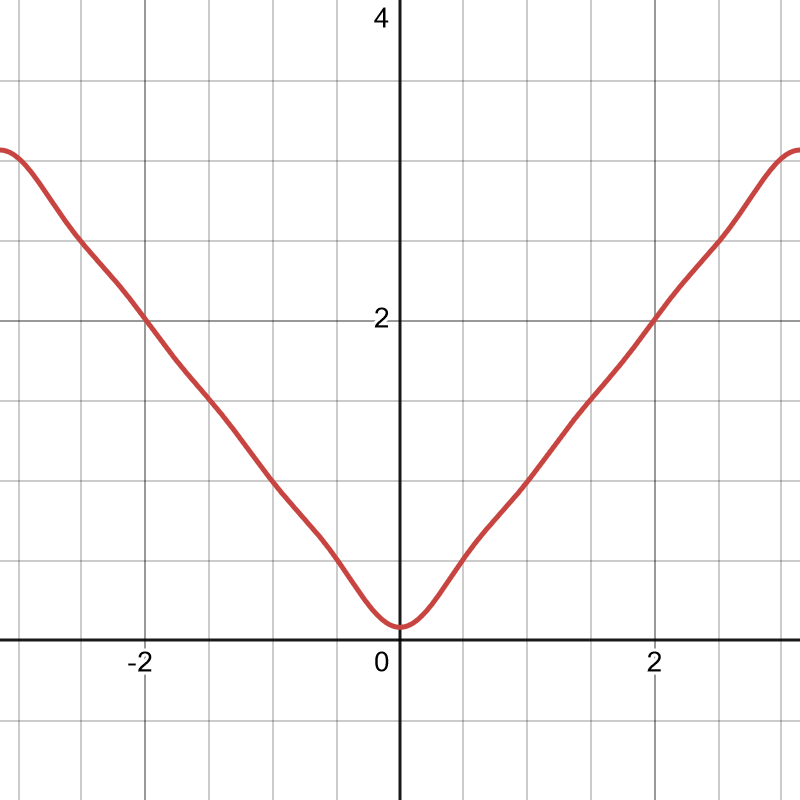
\includegraphics[scale=0.15]{desmos-graph(21).png}
  \caption{Graph of $x\mapsto \frac{\uppi}{2} 
  - \frac{4}{\uppi}
    \sum_{k=0}^3 \frac{\cos((2 k+1) x)}{(2k+1)^2}$
    on the interval $[-\uppi, \uppi]$}
    \end{figure}
  \end{center}
\end{frame}

\begin{frame}{The bigger picture}
  Our basis functions are periodic with period $2 \uppi$. Outside
  the interval $[-\uppi, \uppi]$, our approximation is bad:
  \begin{center}
    \begin{figure}
  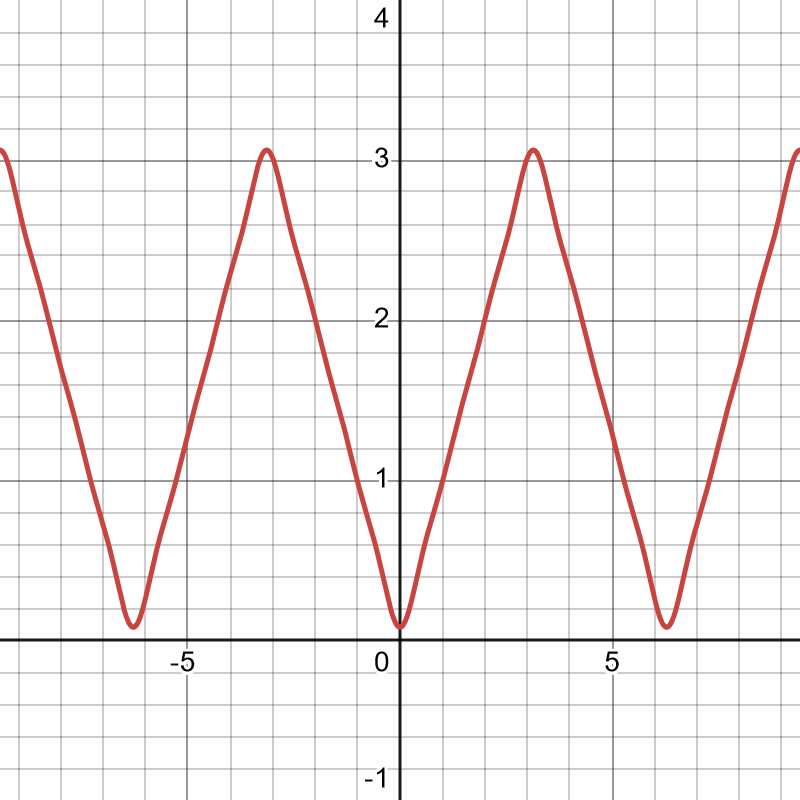
\includegraphics[scale=0.15]{desmos-graph(22).png}
  \caption{Graph of $x\mapsto \frac{\uppi}{2} 
  - \frac{4}{\uppi}
    \sum_{k=0}^3 \frac{\cos((2 k+1) x)}{(2k+1)^2}$
    on the interval $[-3\uppi, 3\uppi]$}
    \end{figure}
  \end{center}
\end{frame}
\end{document}